\documentclass[11pt,two column]{article}
\usepackage{amsmath}
\usepackage{graphicx}
\graphicspath{{Documents/}}
\newcommand{\myvec}[1]{\ensuremath{\begin{pmatrix}#1\end{pmatrix}}}
\let\vec\mathbf
\begin{document}
\title{ASSIGNMENT NO.1  \\COURSE CODE-AI1110\\ Probability And Random Variables }
\author{NAME-Abhishek Kumar ROLL NO.=AI21BTECH11003}
\maketitle
\section*{ Question 1a}
 Solve the following inequation and write down the solution set:\\
\begin{align}
 11x-4 < 15x+4\le13x+14\nonumber,  x\in \mathbb{W}\\\nonumber
\end{align}
Represent the solution on number line .
 \section*{Solution}
There are two inequatilities.\\
\begin{align}
 11x-4 < 15x+4\le13x+14\nonumber,  x\in \mathbb{W}\\
\end{align}
Lets solve for left inequation.
\begin{align}
 11x-4<15x+4\\
 \Rightarrow -8<15x-11x\nonumber\\
 \Rightarrow-2<x\nonumber\\\nonumber
 \end{align}
 Lets solve for right inequation.\\
\begin{align}
  15x+4\le13x+14\\
\Rightarrow 2x\le10\nonumber\\
\Rightarrow x\le5\nonumber\\
 -2 < x\le5,\nonumber\\\nonumber
x\in \mathbb{W}\\\nonumber\\\nonumber\\\nonumber\\\nonumber\\\nonumber
\Rightarrow x=0,1,2,3,4,5 \nonumber
\end{align}
VECTOR WAY TO FIND INTERSECTION POINTS\\\\\\\
vector equations of lines:
\begin{align}

 L1 \equiv \begin{equation} 11x-4-y1=0\hspace{50}  \end{equation}\\\\\\ 
L2 \equiv \begin{equation} 15x+4-y2=0\hspace{50} \end{equation}\\\\\\
L3 \equiv\begin{equation} 13x+14-y3=0\hspace{50} \end{equation}\\\\\\

L1 \equiv \begin{equation} \myvec{11 & -1} \vec{p1}=4\hspace{50}\end{equation}\\
\Rightarrow \myvec{11 & -1} \myvec{x \\ y1}=4\\\\\\\\
L2 \equiv \begin{equation}\myvec{15 & -1} \vec{p2}=-4\hspace{50} \end{equation}\\
\Rightarrow \myvec{15 & -1} \myvec{x \\ y2}=-4\\\\\\\\
L3 \equiv \begin{equation}\myvec{13 & -1} \vec{p3}=-14\hspace{50}\end{equation}\\
\Rightarrow \myvec{13 & -1} \myvec{x \\ y3}=-14\\\\\\\\

\begin{equation} y1=y2\hspace{50} \end{equation}
\Rightarrow \myvec{11 & -1}\myvec{x\\1}=\myvec{15 & 4} \myvec{x \\ 1}\\
\Rightarrow -8=4x\\
\Rightarrow -2=x\\\\\\


\begin{equation} y2=y3\hspace{50} \end{equation}
\Rightarrow \myvec{15 & 4}\myvec{x\\1}=\myvec{13 & 14} \myvec{x \\ 1}\\
\Rightarrow 2x=10\\
\Rightarrow x=5\\
\end{align}
\clearpage
\begin{figure}
\includegraphics[scale=1]{figure_3.png}
\caption{THREE LINES}
\end{figure}
\clearpage
\begin{figure}
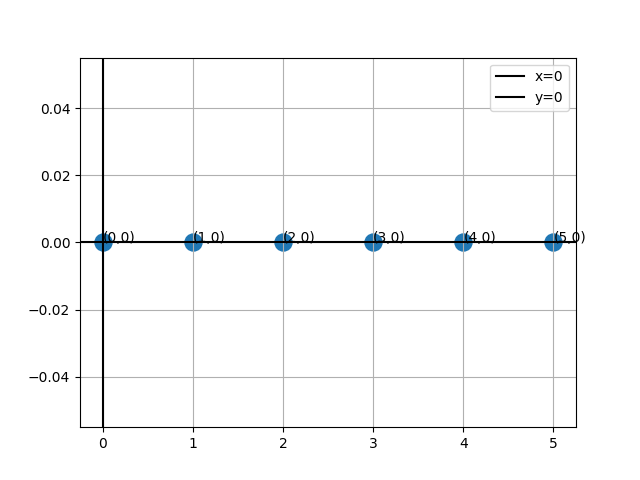
\includegraphics[scale=1]{Figure_4}
\caption{REQUIRED POINTS}


\end{figure}

\end{document}
